\chapter{Simulations Results}
\section{$Re_{\tau}=180$ simulation}

The $Re_{\tau}=180$ simulation has been used to validate our results against the~\cite{kim_moin_moser} ones. \par
The graphs~\ref{loglaw_180} and~\ref{budget_180} show the behavior of the $\bar{u}^{+}$ and the roots means squares in the near wall region, with $\bar{u}^{+}$ indicating the mean velocity profile, expressed in function of the wall units. \par
In both figures we reported the \emph{Kim et al.} results, using dotted line, for comparison. \\~\par

\begin{figure}
\begin{center}
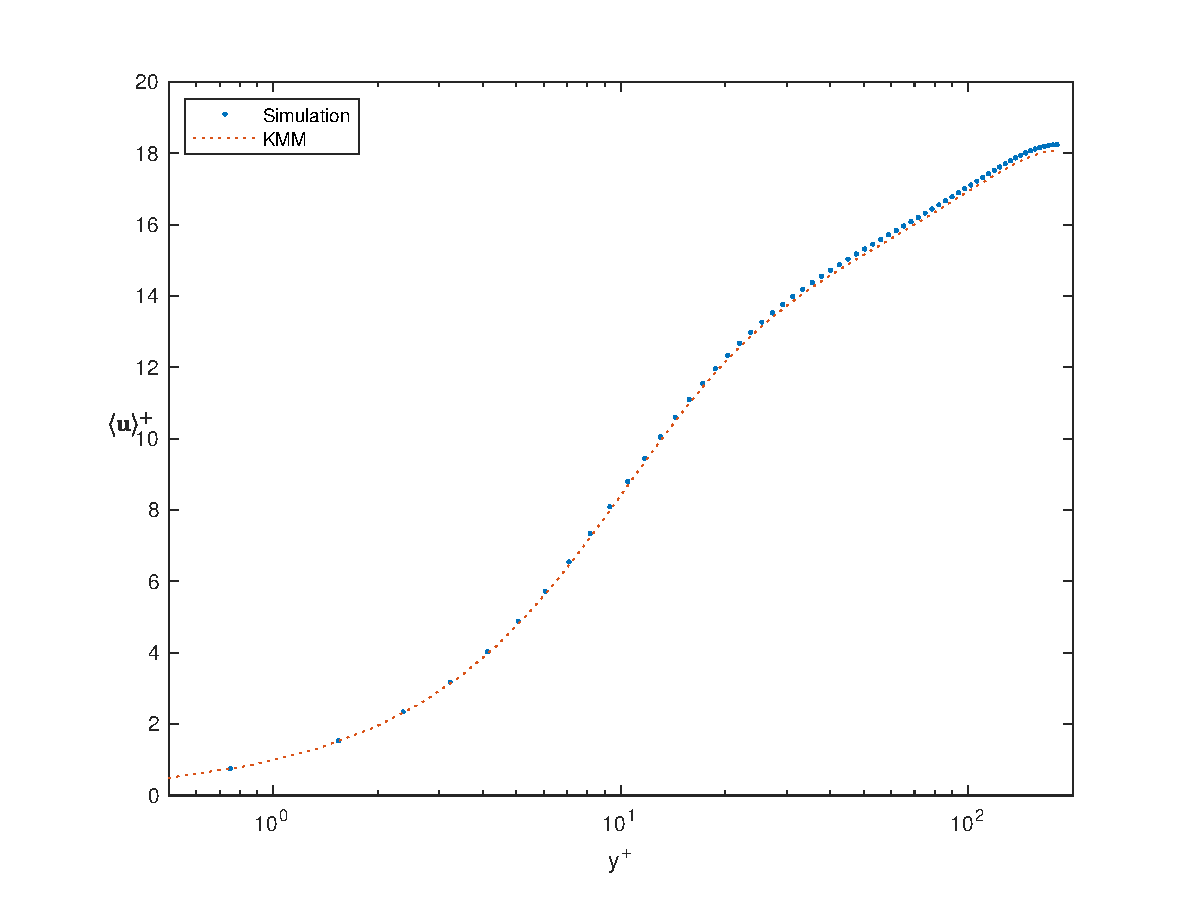
\includegraphics[scale=0.55]{grafici/loglaw_180.eps}
\caption{$\bar{u}^{+}$ in the near wall region for a $Re_{\tau}=180$ simulation}
\label{loglaw_180}
\end{center} 
\end{figure}

\begin{figure}
\begin{center}
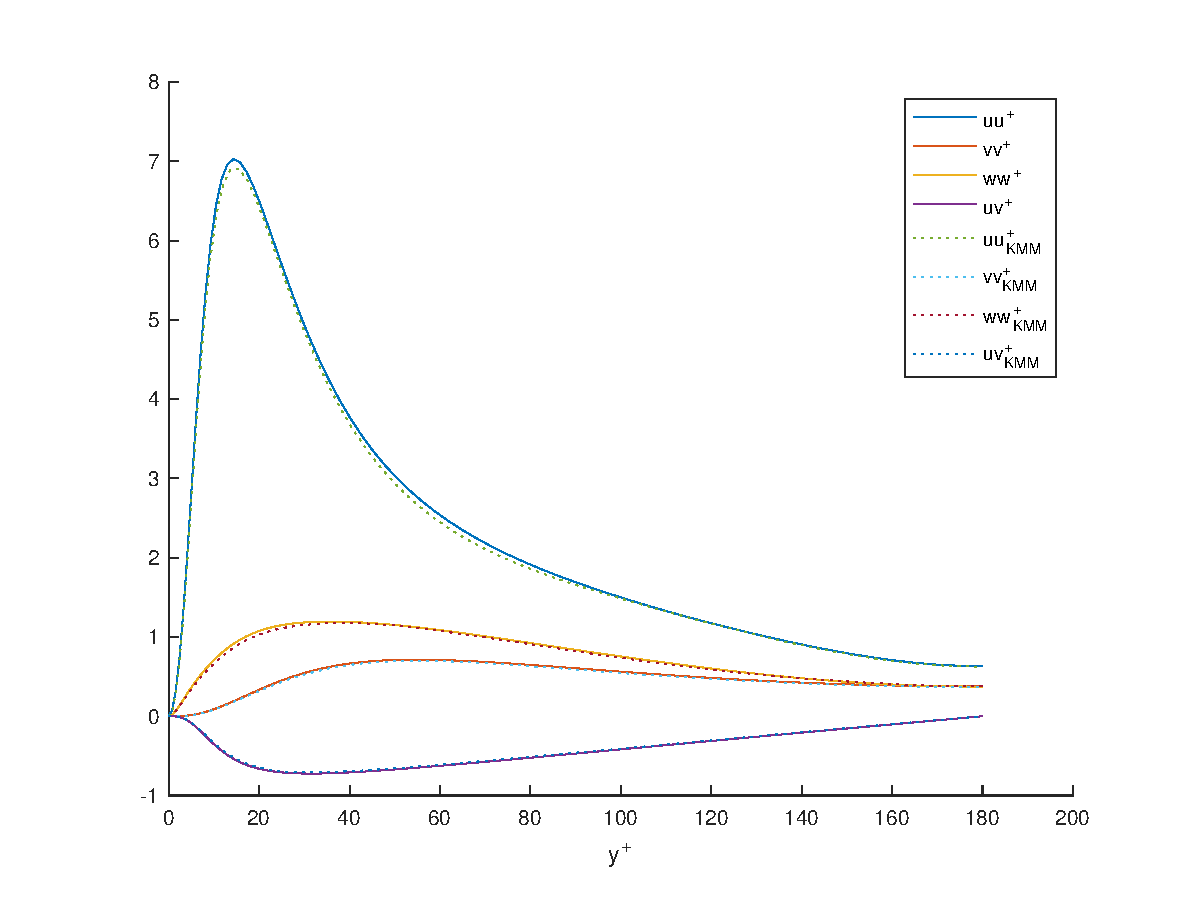
\includegraphics[scale=0.55]{grafici/budget_180.eps}
\caption{rms terms for a $Re_{\tau}=180$ simulation}
\label{budget_180}
\end{center} 
\end{figure}


Our statistics have been registered using a simulation time of 50 non dimensional units, sampling data every 0.1 steps.
In total 500 fields have been used to perform the ensemble average. \par

The data fitting is good, despite being perfect. The divergences among our database and the~\cite{kim_moin_moser} ones are possibly due to the fluctuations, rounding errors and differences in averaging times.\\~\par

Nevertheless the results are in agreement with the typical curves behavior, in particular, by looking at the root mean square curves, we can clearly see that $\langle uu\rangle$ and $\langle ww\rangle$ depart from 0 as $y^{2}$, while $\langle uv\rangle$ and $\langle vv\rangle$ increase more slowly, as $y^{3}$ and $y^{4}$, in agreement with~\cite[284]{pope}.
All these information testify that, close to the walls, there is a \emph{two component flow}, with $v=0$ whereas $u$ and $w$ are non-zero. The resulting motion corresponds to flow in planes parallel to the wall. \\~\par

The figure~\ref{loglaw_180} report the $\bar{u}^{+}$ behavior near the wall. From 0 up to 5 $y^{+}$ units we can see the typical $\bar{u}^{+}=y^{+}$ behavior, which characterize the viscous sublayer. Once $y^{+}>30$ we see the arise of the logarithmic law of the wall, characterized by the equation

\begin{equation*}
\bar{u}^{+} = \frac{1}{\kappa} \ln y^{+} +C^{+},
\end{equation*}


\begin{figure}
\begin{center}
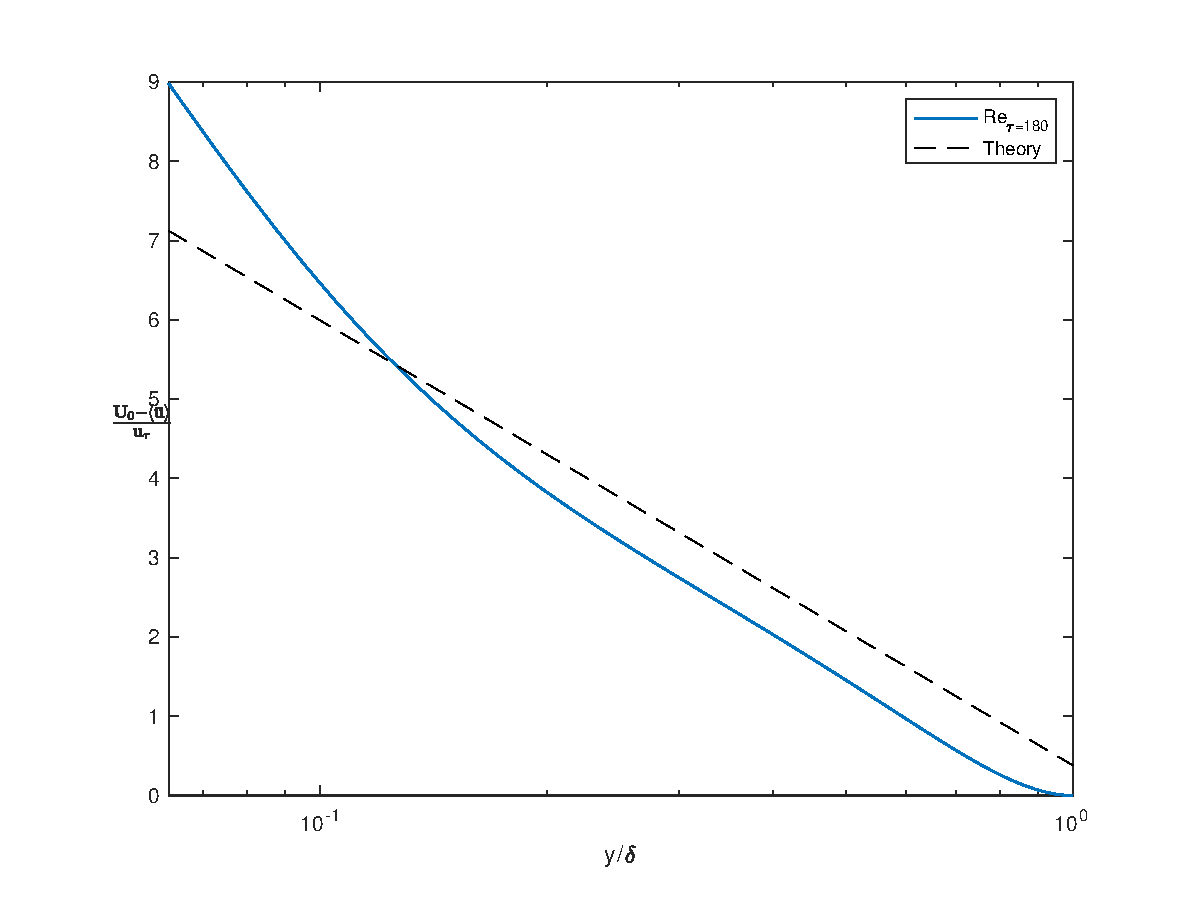
\includegraphics[scale=0.55]{grafici/velocity_defect_180.eps}
\caption{Velocity defect for a $Re_{\tau}=180$ simulation}
\label{velocity:defect:180}
\end{center} 
\end{figure}

where the constants $\kappa=0.41$ and $C^{+}\approx 5.2$, like smooth wall experiments, made by Von Karman, evidenced. \par
This velocity profile is typically denoted as \emph{the law of the wall}, and has been postulated by Prandtl in 1925.\par
Far away from the wall, the implications of the previous law originate the so called \emph{velocity defect}.
Our experimental data fits the theory, as figure~\ref{velocity:defect:180} suggest.\\~\par

On page~\pageref{k+budgets:180} is possible to look at the plot of the turbulent kinetic energy with the \emph{rms} terms, next to the plot of the \emph{production term}, estimated assuming boundary layer approximations, in which we neglect the contributions of all mean velocities gradients, except for $\frac{\partial{\bar{u}}}{\partial{y}}$, so the production term of the TKE can be expressed as $P=-\langle uv\rangle \frac{\partial{\bar{u}}}{\partial{y}}$.\par
The image~\ref{k+budgets:180} highlight that the energy associated with the turbulence tends to develop close to the walls, and lose effectiveness once departing from there.\par
The \emph{production term} is part of the so called turbulent kinetic energy budgets and plays a key role in the interaction of the mean energy equation and TKE. The action of the mean velocity gradients working against the Reynolds stresses removes kinetic energy from the mean flow and transfers it to the fluctuating velocity field. \par
Despite the approximation, the effect of such term is well depicted, with its contribution concentrated near the walls, with the peak around $y^{+} \approx 12$, and becomes zero approaching the half channel height. \\~\par

\begin{figure}
\begin{center}
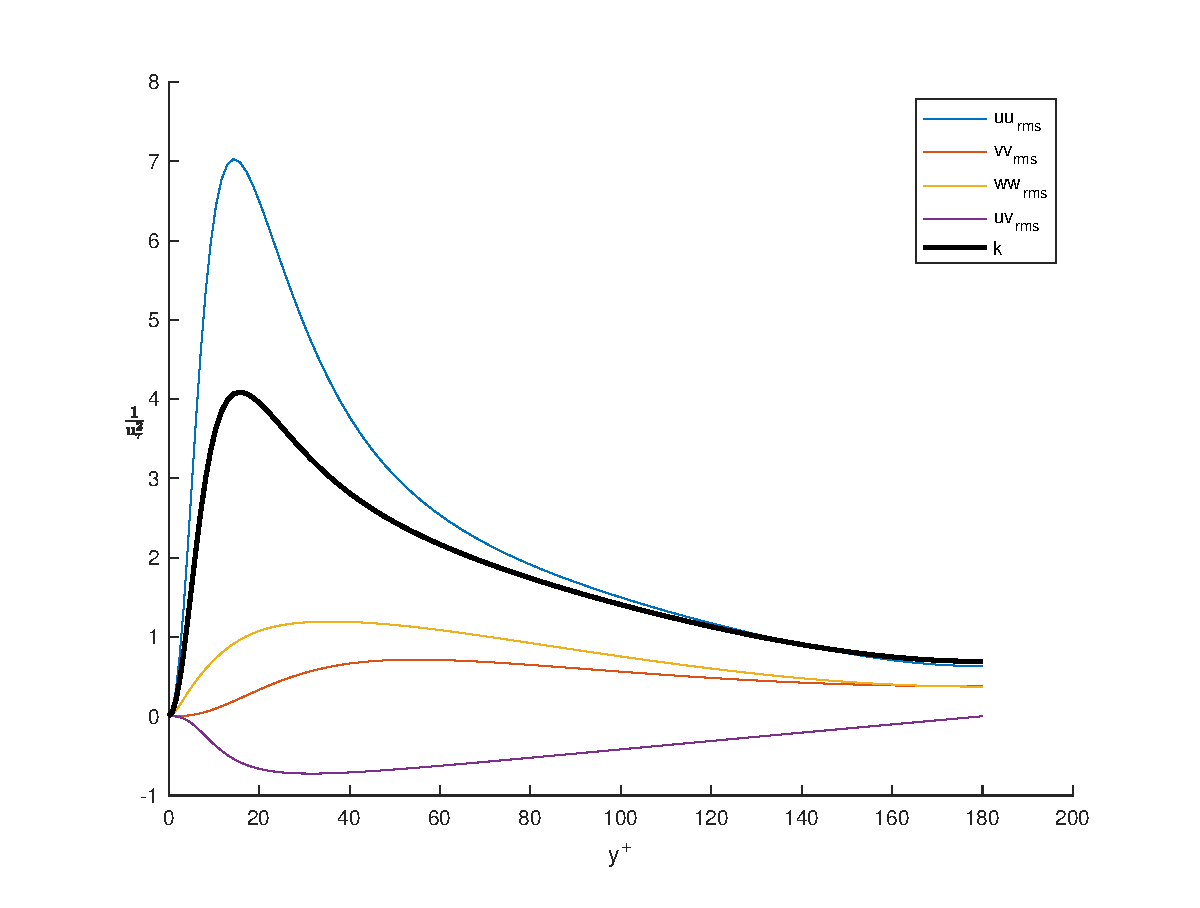
\includegraphics[scale=0.55]{grafici/budget+k_180.eps}
\caption{TKE and rms terms for a $Re_{\tau}=180$ simulation}
\label{k+budgets:180}
\end{center} 
\end{figure}

\begin{figure}
\begin{center}
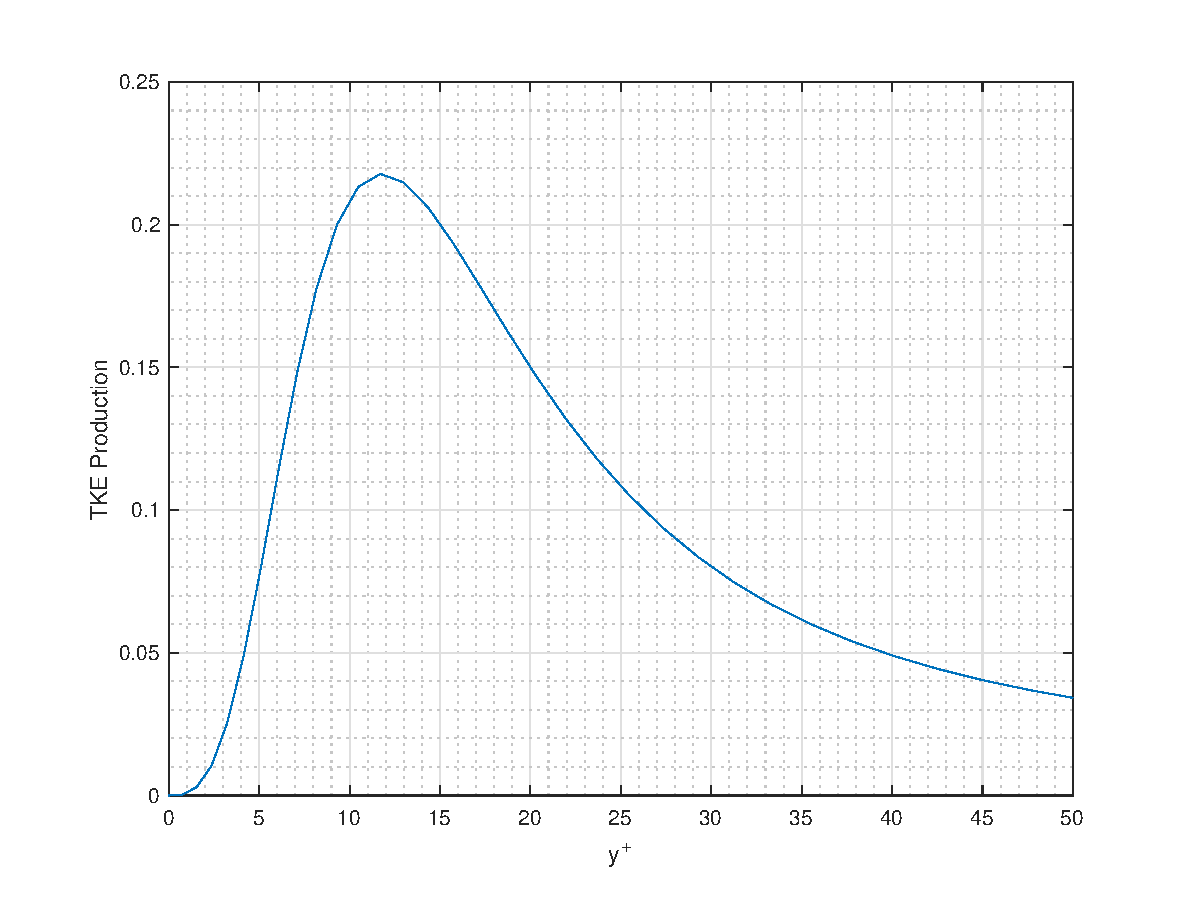
\includegraphics[scale=0.55]{grafici/tke_prod_180.eps}
\caption{Production term of the TKE eq. for a $Re_{\tau}=180$ simulation}
\label{tke:prod:180}
\end{center} 
\end{figure}

The \emph{production} peak can be estimated also by looking at where the Reynolds stresses becomes equal to the viscous ones.
On figure~\ref{stresses:180} we reported the plot of the normalized total shear stress, with its contribution, where is possible to see that the two curves overlap for $y\approx 12$.\par


\begin{figure}
\begin{center}
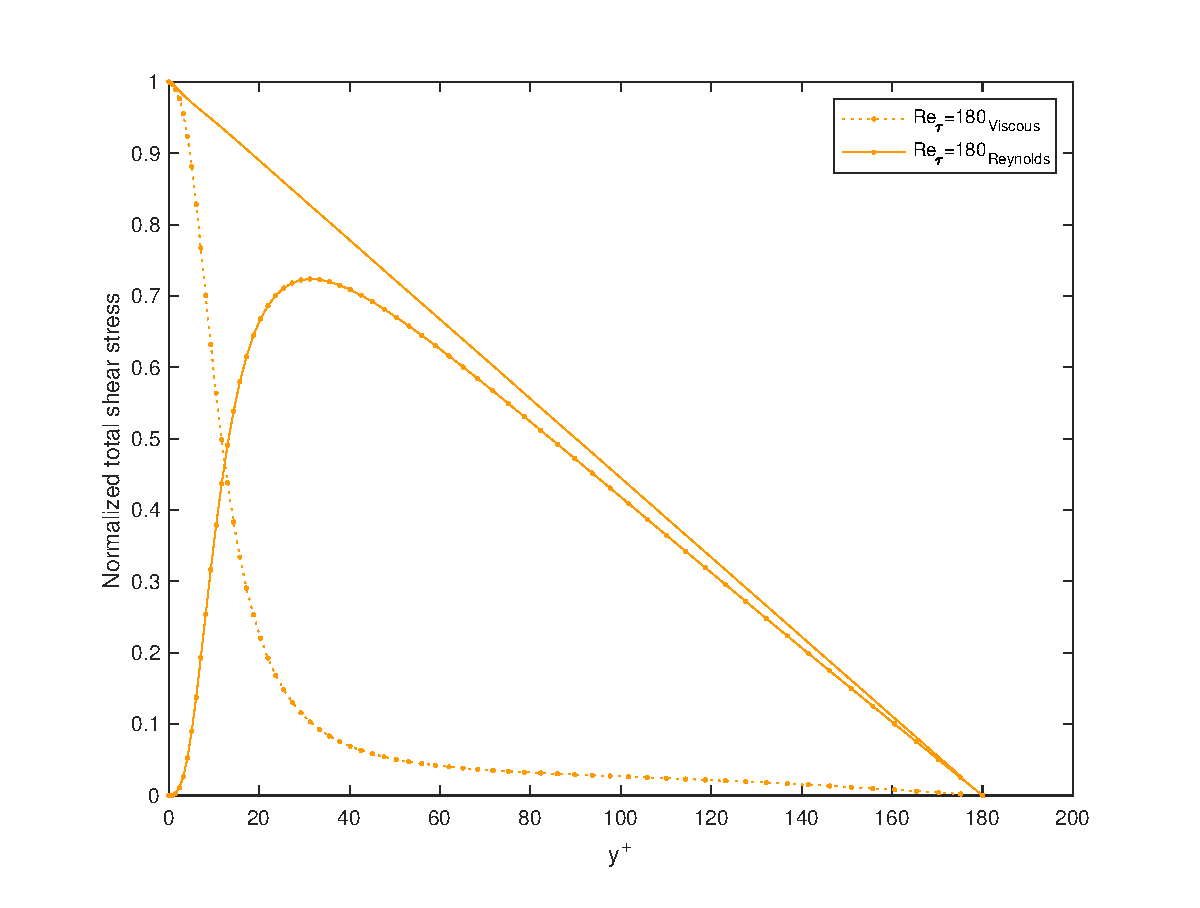
\includegraphics[scale=0.55]{grafici/stresses_180.eps}
\caption{Normalized total shear stresses for a $Re_{\tau}=180$ simulation}
\label{stresses:180}
\end{center} 
\end{figure}